\chapter{Sensitivity-aware motion planner}
\markboth{Sensitivity-aware motion planner}{}% To set left/right header
% \localtableofcontents

This chapter introduces the first major contribution of this thesis, by leveraging the sensitivity concept discussed in Chapter~\ref{chap:models}.
The contribution of this chapter is twofold:
\begin{enumerate}
    \item Firstly, it addresses the generation of a desired trajectory with minimal sensitivity, ensuring that the closed-loop evolution of $\q(t)$/$\u(t)$ closely matches its nominal evolution, $\q_n(t)$/$\u_n(t)$. While previous work has explored sensitivity optimization for generating locally sensitivity-optimal trajectories \cite{cPi, cTh}, this approach has never been applied within a global sampling-based planning framework that accounts for obstacles. Therefore, the first contribution is to propose methods for efficiently performing global sensitivity-optimal motion planning.
    \item Secondly, this chapter introduces, for the first time, the use of sensitivity-based uncertainty tubes to enforce constraints in both the state and input spaces. This enables the generation of intrinsically-robust motions (i.e. accounting for the controller's behavior with respect to uncertainty) that ensures robustness to both the environment and the actuator limits.
\end{enumerate}
This chapter is organized as follows: it first presents in Section~\ref{sec:metrics} how the uncertainty tubes of Section~\ref{sec:tubes} are used to enforce robust constraints in the planning process, as well as the development of an appropriate cost function for performing global sensitivity optimization.
Then, in Section~\ref{sec:unified}, a unified approach is presented, which allows for planning a robust trajectory with optimal sensitivity by directly incorporating the sensitivity computation into the optimal tree-building process (e.g., \myglsentry{rrtstar}). 
This approach is tested on the robot models described in Chapter~\ref{chap:models} showing poor scalability to the system complexity.
Finally, a decoupled approach that shows better efficiency for more complex systems, is introduced in Section~\ref{sec:decoupled}, followed by conclusions in Section~\ref{sec:concl}.

This chapter is associated to the following publication in ICRA 2023: Wasiela, S., Giordano, P. R., Cortés, J., and Simeon, T. (2023, May). "A sensitivity-aware motion planner (samp) to generate intrinsically-robust trajectories." In IEEE International Conference on Robotics and Automation (ICRA) (pp. 12707-12713).

\section{??Sensitivity-aware metrics??}\label{sec:metrics}

This section first presents how the uncertainty tubes from Section~\ref{sec:tubes} are used to perform robust feasibility checks, followed by the selection of an appropriate cost function for global sampling-based optimization.

\subsubsection{Robust feasibility check}\label{sec:robust_CC}

As previously mentioned in Chapter~\ref{chap:related_work}, sampling-based algorithms generate global trajectories by combining multiple continuous local trajectories.
During the process, each of these local trajectories are subject to collision checks to determine their feasibility.
However, in this thesis, the collision check is extended to include a more general feasibility test, which also accounts for the control input space. 
This extension ensures that the generated trajectories are not only free from obstacles but also prevent control inputs from reaching saturation. 
Additionally, it accounts for uncertainty in both the state and control input spaces, further enhancing the robustness of the trajectories.
The following sections describe how these extended feasibility checks are performed to ensure the robustness of each local trajectory in this context.
It is important to note that these tests are not continuous; rather, they are performed along a discrete representation of the local trajectories.

\paragraph{Robust collision checking}
In this thesis, collision detection is performed using the widely used C implementation of PyBullet~\cite{cBullet}, which operates as follows: 
\begin{enumerate}
    \item It starts with a broad-phase collision detection using \myglsentry{AABBs} to quickly eliminate pairs of objects that are too far apart to collide, allowing the more computationally intensive collision checks to focus only on pairs that are potentially close to each other.
    \item Then, it performs a narrow-phase collision detection that, after potential collision pairs are identified, checks for each pair. For each identified potential collision pair, this phase uses a more precise robot representation (as defined by the user) and specialized collision algorithms to detect actual intersections and determine contact points, normals, and penetration depths.
\end{enumerate}

Extending this procedure to account for robot state uncertainty aims to verify that the resulting extended bounding volume, which the robot may occupy due to the uncertainty, is clear of obstacles.
In this thesis, such bounding volume is computed by considering only the uncertainty in the linear position subspace for simplicity (i.e., the $x,y,z$ subspace for the quadrotor applications or the $x,y$ subspace for the differential drive robot applications).
Several strategies are evaluated based on their computational efficiency, conservatism, and library capabilities:
\begin{enumerate}
    \item The simplest method to account for position uncertainty in collision checking is to compare the distance between the current robot AABB and the nearest obstacle, incorporating the maximum possible deviations by using the worst-case uncertainty tube radius from Equation~\ref{eq:radius} (see~\ref{chap:appendixA} for proof).
    This check corresponds to a uniform scaling of the AABB by the maximum uncertainty radius as depicted in Figure~\ref{fig:CC1}. 
    Since the C PyBullet library does not support re-scaling an existing collision shape on the fly, a new shape must be created whenever scaling is required. 
    By using this straightforward distance check, one can avoid the need to create new shapes.
    However, this method represent a conservative approach as all directions are scaled in the same way.
    \item As mentioned above, a less conservative approach involves creating an extended AABB by scaling the current robot AABB in all directions according to their respective uncertainty radii as shown in Figure~\ref{fig:CC2}. 
    However, this method requires the creation of a new collision shape for each collision test.
    \item The approaches mentioned above, though efficient, are conservative because they only use the current robot AABB and do not leverage narrow-phase collision checks that consider the precise robot mesh representation. 
    However, generating the accurate extended collision shape that incorporates uncertainty, required for the second phase, is challenging, as the library supports only standard primitives like boxes, spheres, cylinders, etc.
    To address this, the third approach approximates the extended collision shape by sampling on the surface of the uncertainty ellipsoid bounding box defined by the uncertainty tube radii, rather than creating a new collision shape (see Figure~\ref{fig:CC3}). 
    While this method more accurately approximates the true extended collision shape than the two first approaches, it requires multiple calls to the collision-checking function for each robot state tested.
\end{enumerate}

\begin{figure}[t]
    \centering
    % Row 1
    \begin{subfigure}{0.4\textwidth}
        \centering
        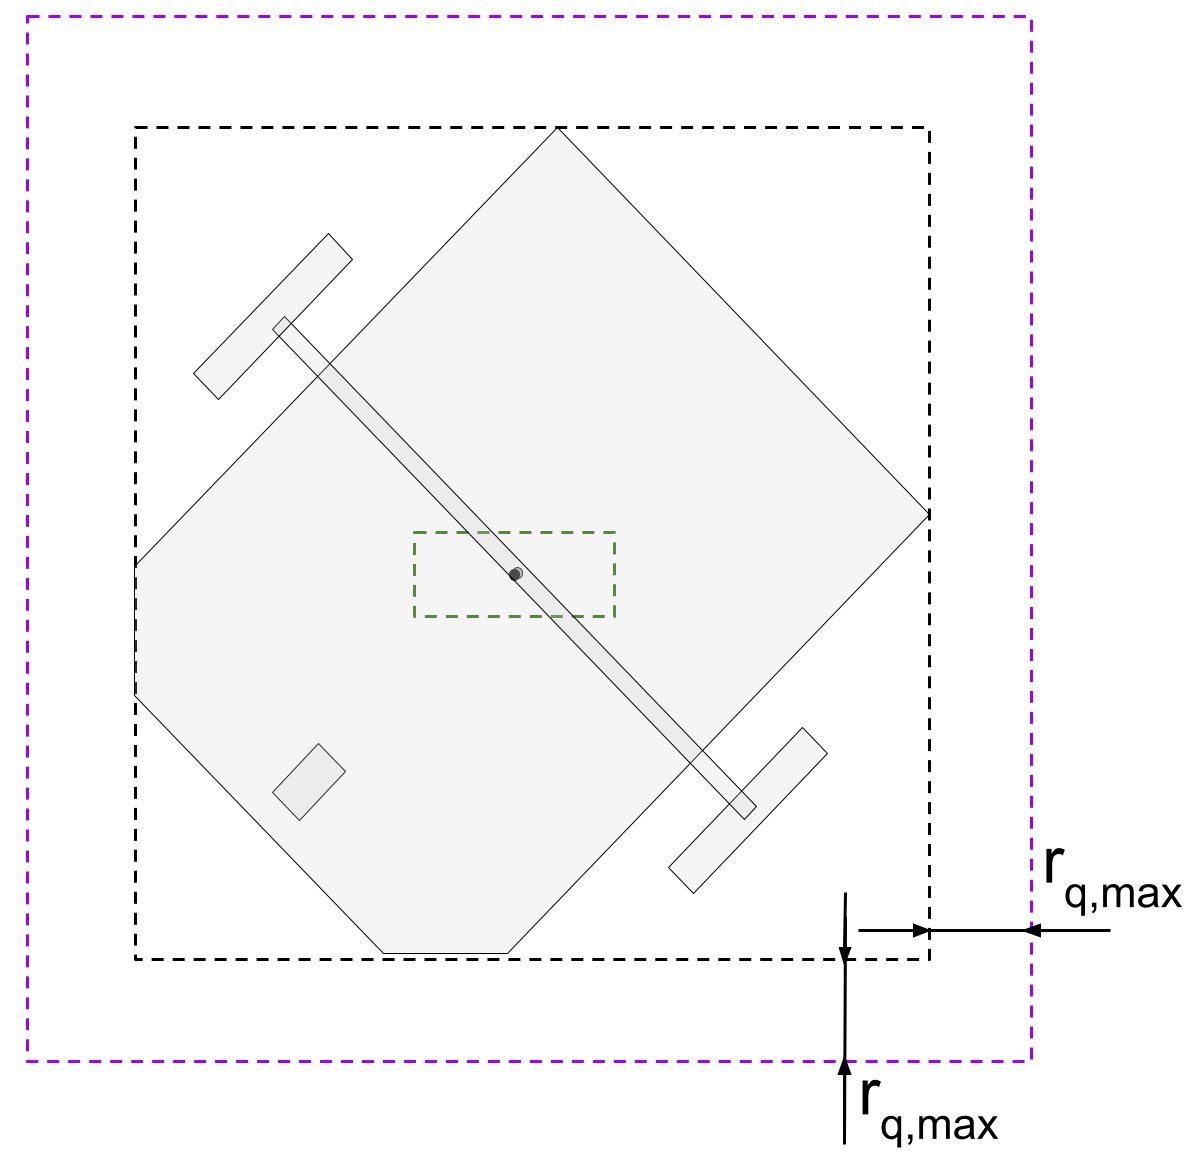
\includegraphics[width=\linewidth]{figures/samp/CC1.png}
        \caption{}
        \label{fig:CC1}
    \end{subfigure}
    % \hfill
    \begin{subfigure}{0.4\textwidth}
        \centering
        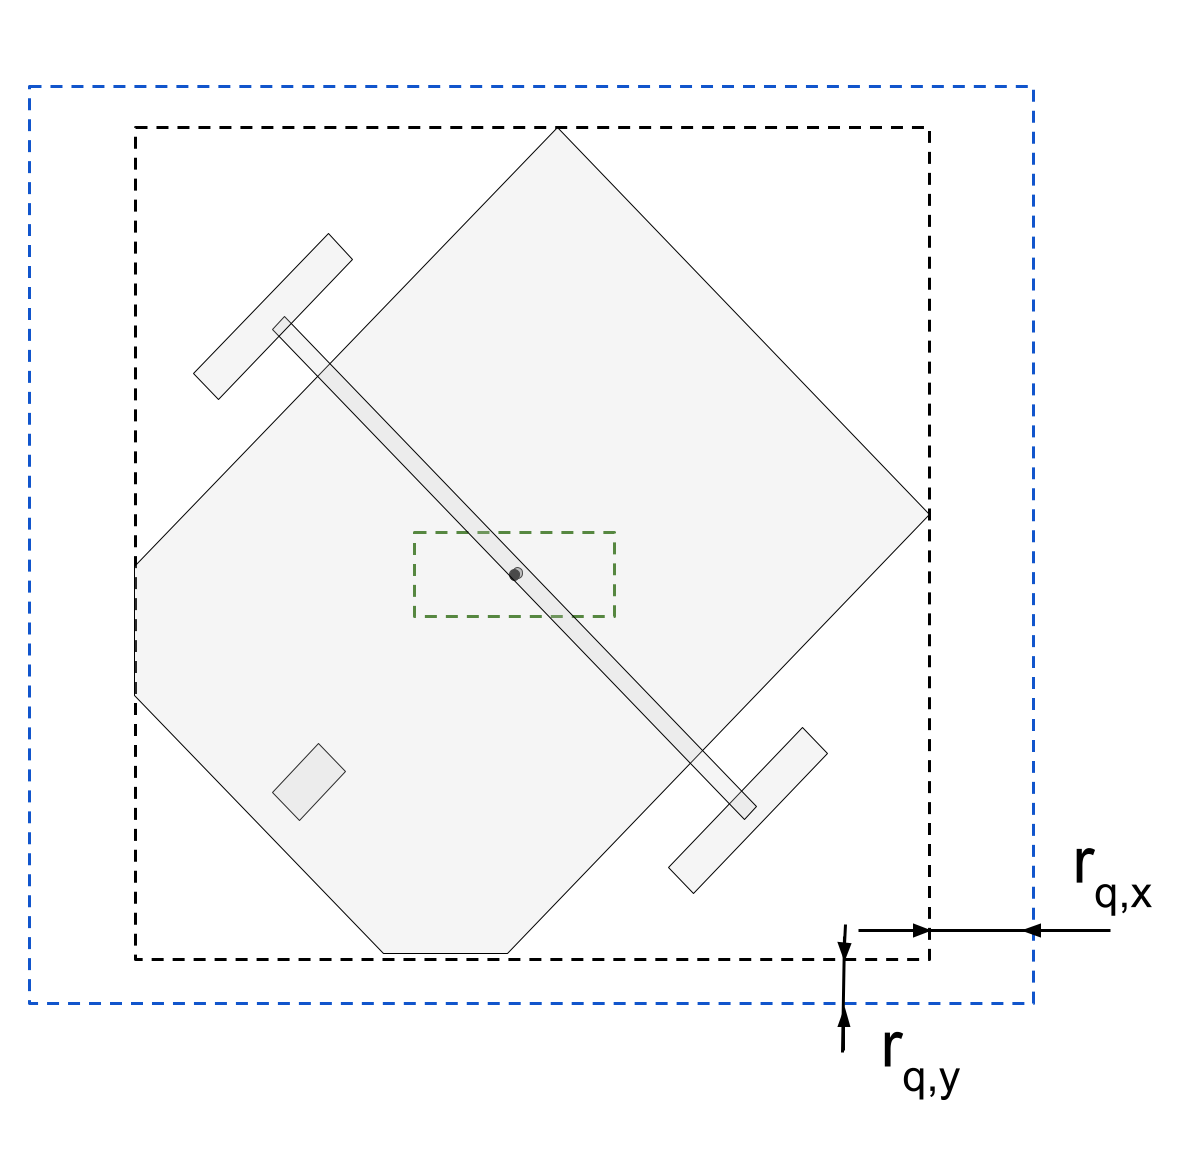
\includegraphics[width=\linewidth]{figures/samp/CC2.png}
        \caption{}
        \label{fig:CC2}
    \end{subfigure}
    
    % Row 2
    \begin{subfigure}{0.4\textwidth}
        \centering
        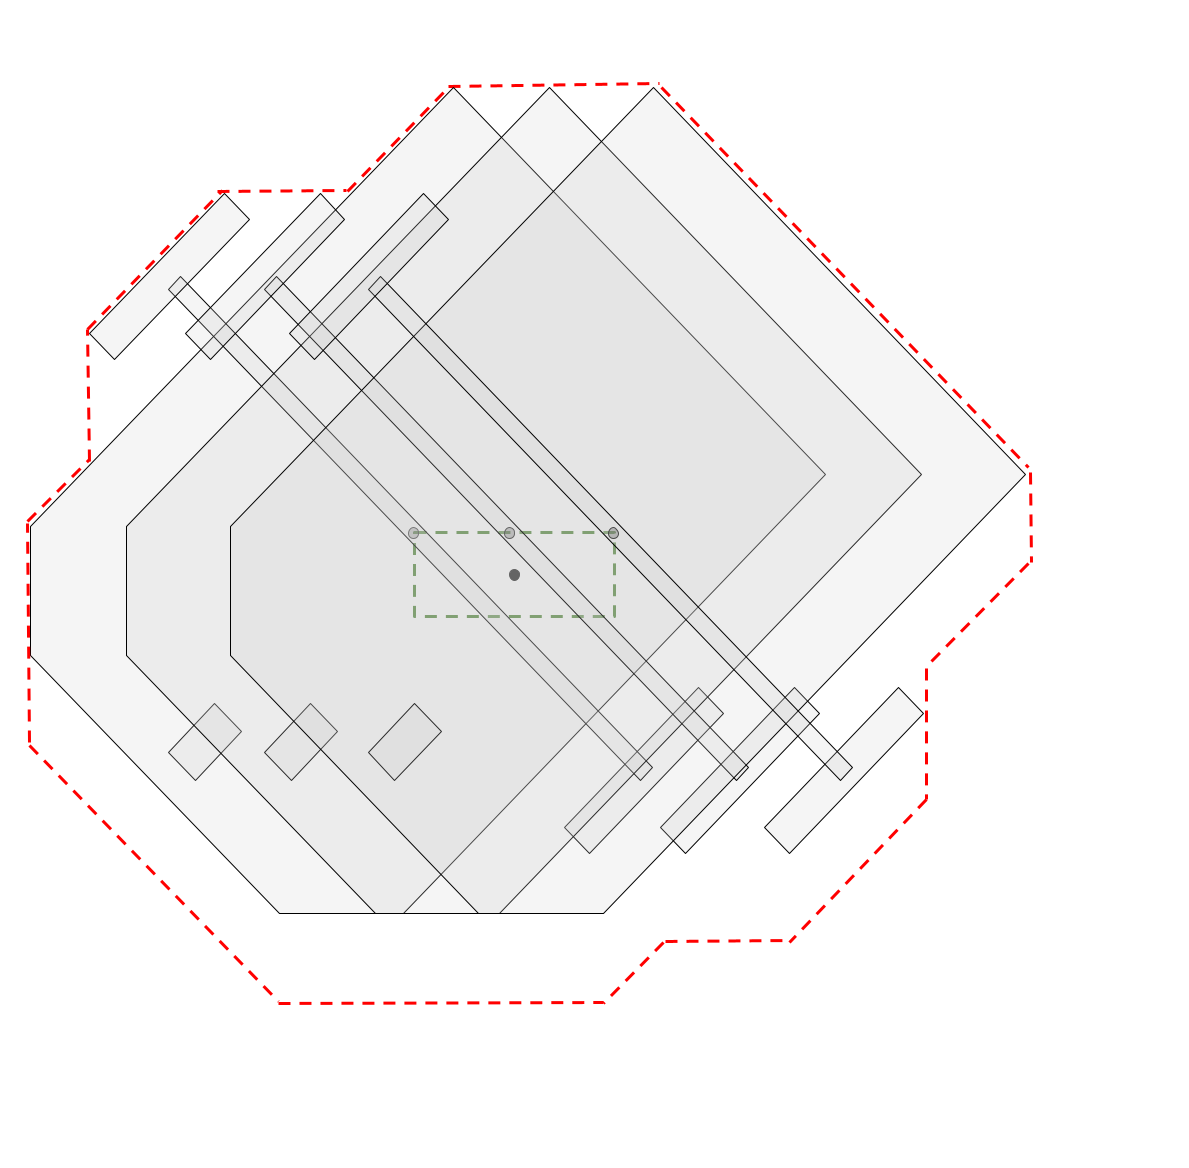
\includegraphics[width=\linewidth]{figures/samp/CC3.png}
        \caption{}
        \vspace{-0.3cm}
        \label{fig:CC3}
    \end{subfigure}
    % \hfill
    \begin{subfigure}{0.4\textwidth}
        \centering
        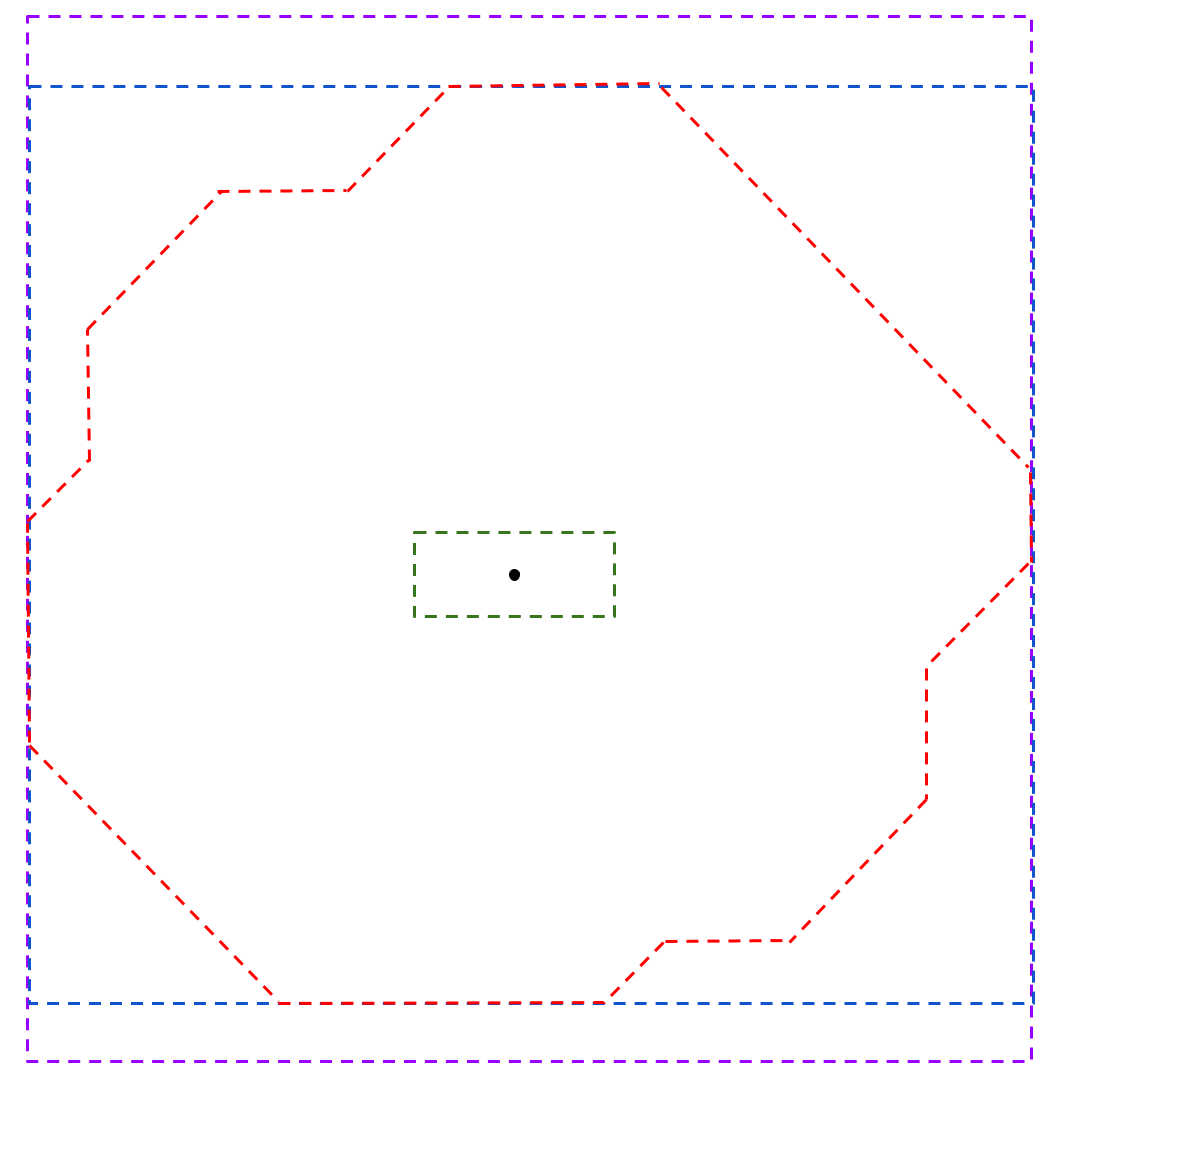
\includegraphics[width=\linewidth]{figures/samp/CCall.png}
        \caption{}
        \vspace{-0.3cm}
        \label{fig:CCall}
    \end{subfigure}

    \caption{Figure showing the space covered by each of the three methods: (a) uniformly scaled AABB, (b) extended AABB, and (c) sampling-based approximation of the extended collision shape, for a differential drive robot with its associated uncertainty ellipsoid bounding box (green) based on computed uncertainty radii. Comparison of the three methods is shown in (d).}
    \label{fig:CCmethods}
\end{figure}

These different approaches enable progressively more precise collision testing, from the first to the third method, as illustrated in the Figure~\ref{fig:CCall} that shows a comparison of the resulting tested collision shapes according to the aforementioned methods for the 2D differential drive robot.
However, this increased accuracy comes at the cost of longer computational times, as noted earlier. 
To quantify this, the mean running time of each method was evaluated based on 1.000 robust collision tests performed using the quadrotor model described in Section~\ref{sec:quad_model}. 
The results indicate that the first method, which involves a simple distance check, has an average runtime of 3 microseconds. 
The second method, which creates an extended uncertain AABB, takes 7 microseconds to compute. 
Finally, the method that approximates the true extended collision shape requires 45 microseconds. 
It is worth mentioning that this last approach involves 14 samples (each corner and the center of each face), and therefore, its runtime can be approximated as linear with respect to the number of samples, compared to a simple test.

Finally, in this thesis, the second approach is used for robust collision checking, as it offers a more precise approximation of the extended collision shape with only a minor increase in computation time than the first approach. 
However, the third approach is employed in the scenario presented in Section~\ref{sec:AOptim}, as it demands a higher level of collision accuracy.
Although the methods employed in this thesis for robust collision checking rely on the uncertainty ellipsoid bounding box computed using Equation~\ref{eq:radius}, the tubes are represented by ellipsoids in the various figures of this manuscript for smoother visualization.

\paragraph{Robust saturation checking}
Then, in this manuscript, the feasibility check is not restricted to the aforementioned collision test presented above, but it also verifies that the robot control inputs does not saturate.
This test is performed by checking that the tube associated with each control input remains in its feasibility domain.
An example of infeasible input for the quadrotor case is presented in Figure.\ref{fig:invalid_inputs},  where the tube (green) around the nominal control input of the first actuator (blue) exceeds the maximum allowed input (red).
Note that this simple test is less costly than the robust collision checking one, it is therefore performed first by mean of computational efficiency. 

\begin{figure} [t]
    \centering
    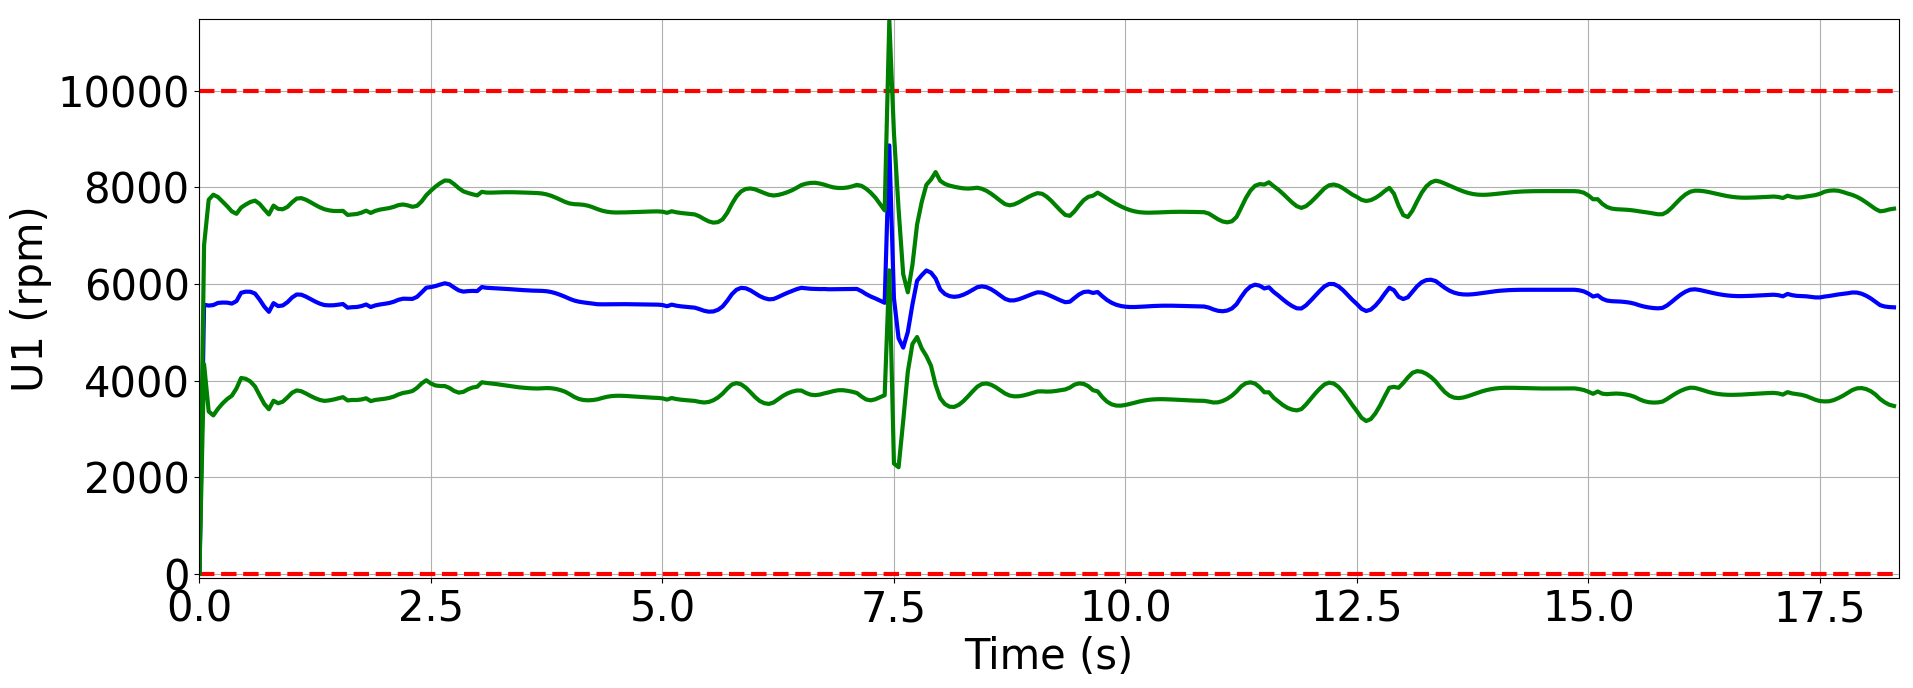
\includegraphics[width=0.8\linewidth]{figures/samp/Invalid_Inputs.png} 
    \caption{Non-robust nominal control input profile for the first rotor of a quadrotor (blue) along a specified trajectory, depicted with its uncertainty tube (green) and the control inputs limits (red).}%
    \label{fig:invalid_inputs}%
\end{figure}

\subsubsection{Cost function}\label{sec:sensi_cost}

\begin{figure} [t]
    \centering
    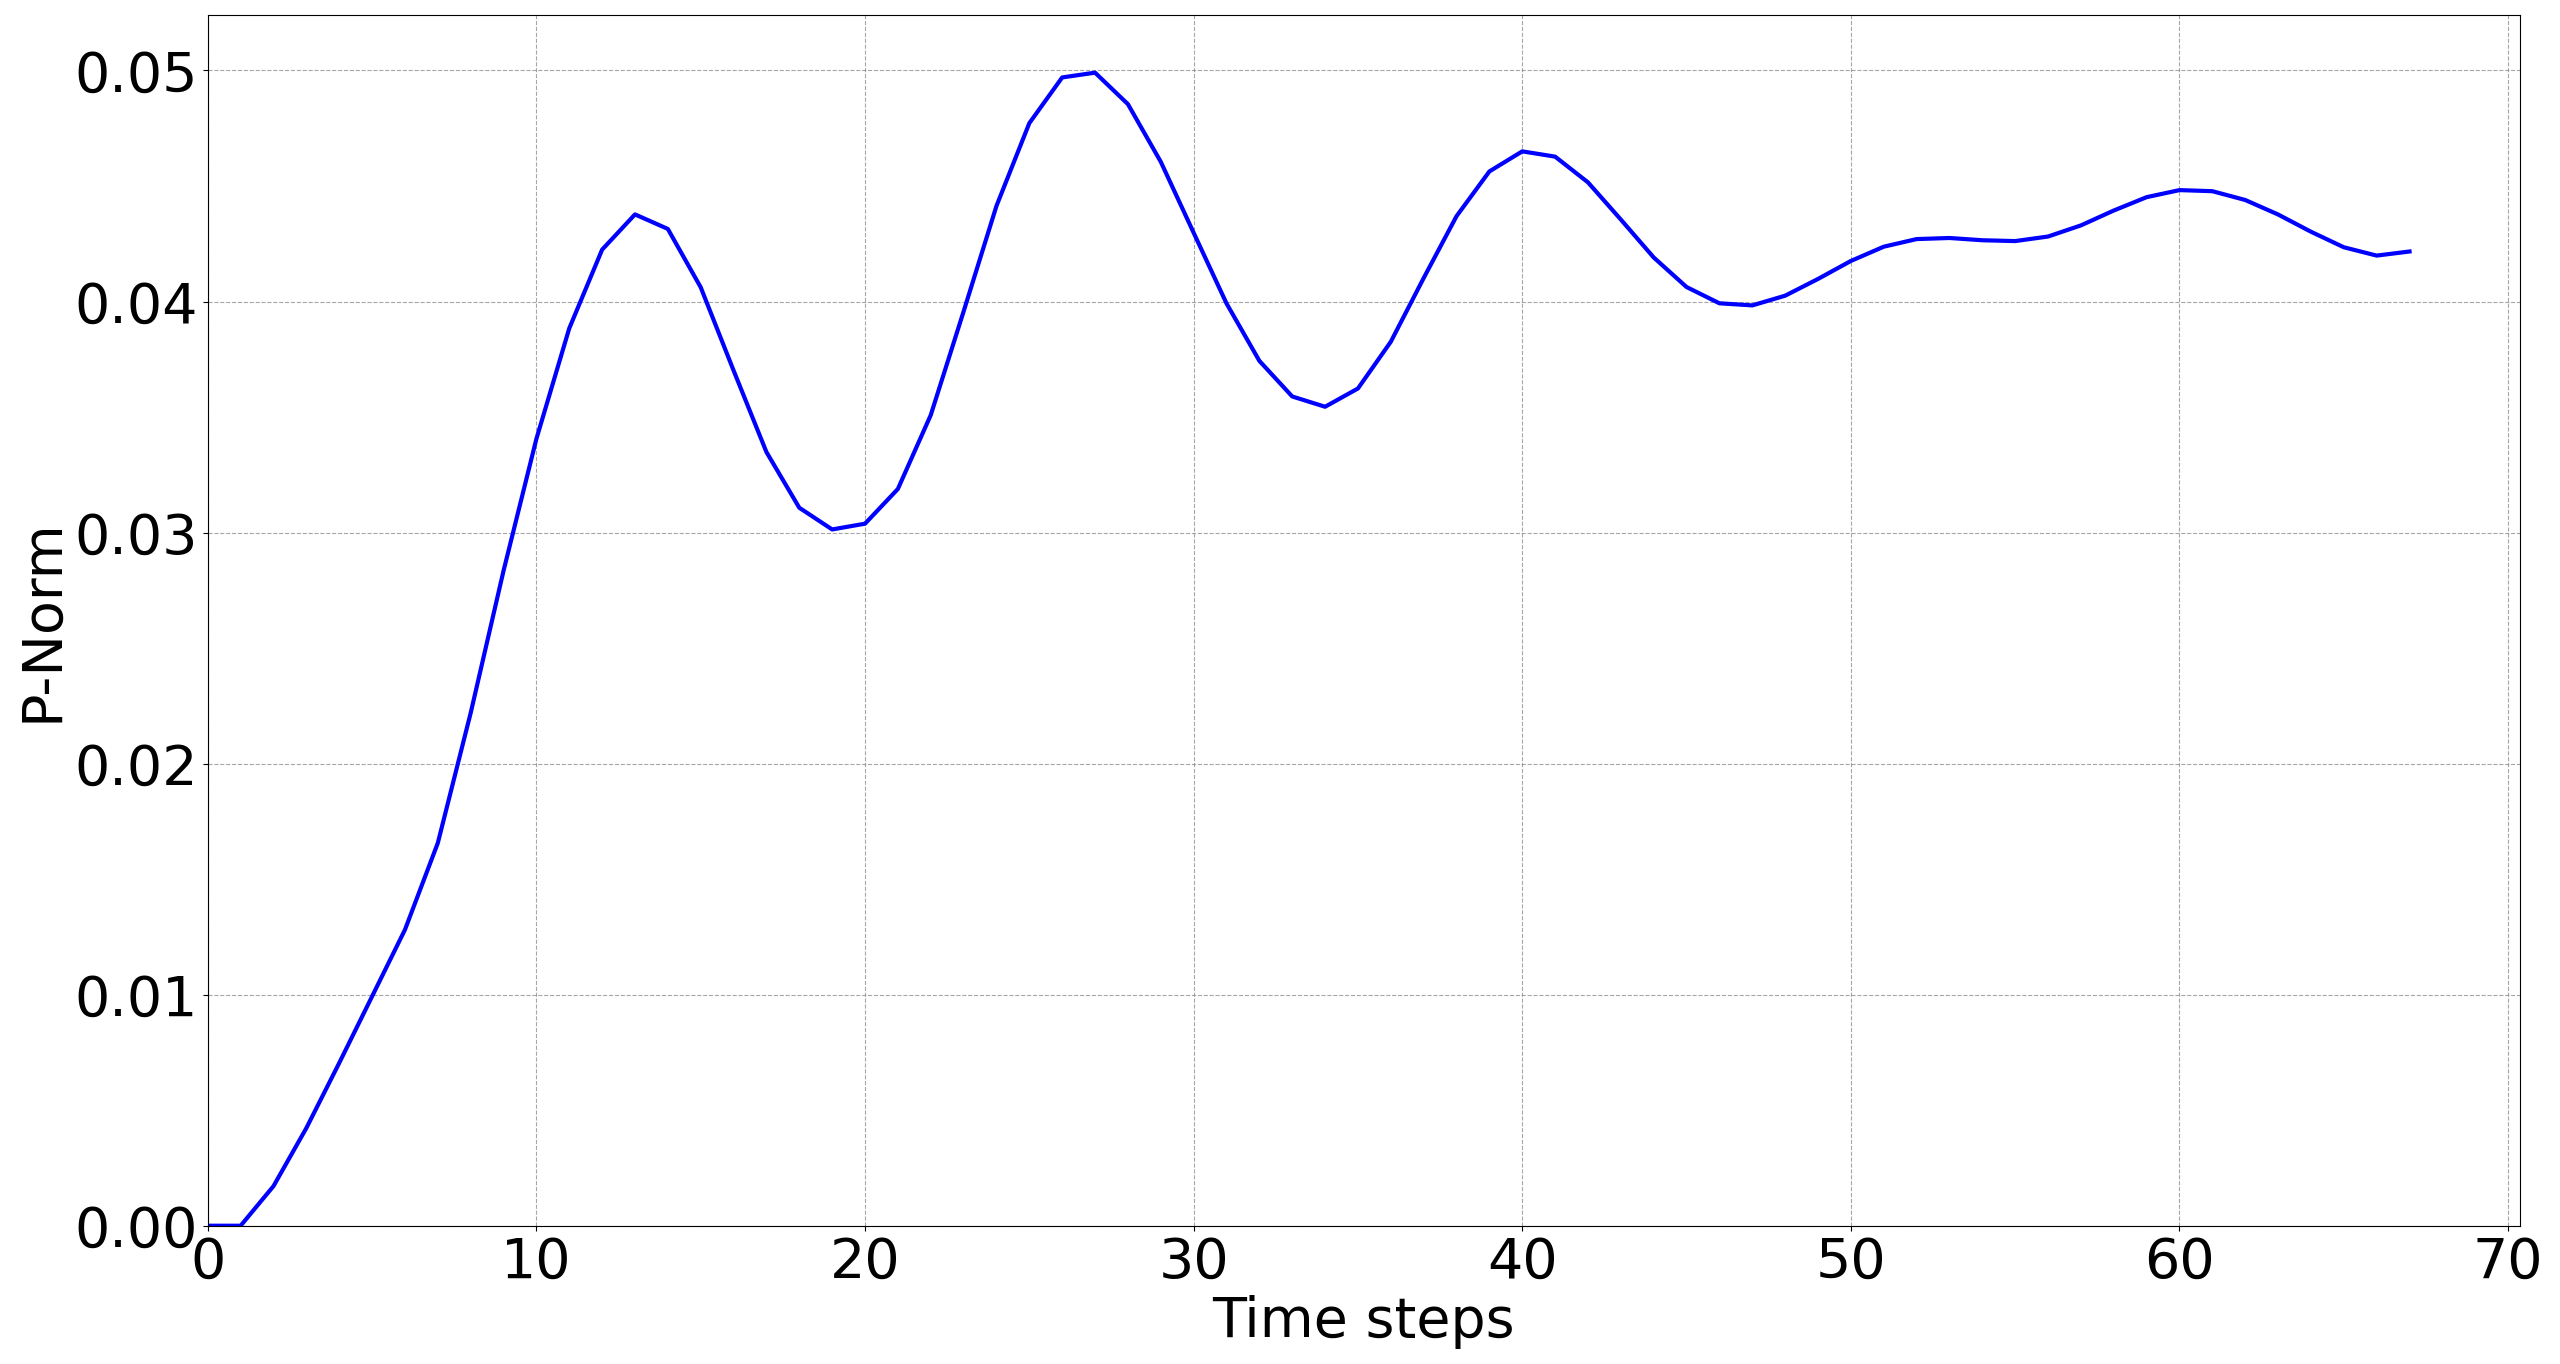
\includegraphics[width=0.8\linewidth]{figures/samp/non_monotoic.png} 
    \caption{Non monotonic p-norm profile along a 70-state trajectory for a quadrotor example.}%
    \label{fig:monotonic}%
\end{figure}

Now that the sensitivity matrices are defined, one can compute and minimize a chosen norm of $\bPi(t)$ and $\bTheta(t)$ w.r.t. the desired trajectory $\q_d(t)$.

However, sensitivity non monotonic and non additive, not suitable for optimal motion planning that requires monotonic and additive cost function properties.
Add figure.

We therefore chose integral.
However, instead of integral of norm of PI as done in~\cite{cPi,cTh}, we chose integral of p-norm radii, better capture deviations to the nominal case.

\section{Unified approach}\label{sec:unified}

This section first present a unified approach that allow planning a robust trajectory with an optimal sensitivity by directly incorporating the sensitivity computation in an optimal planning process (e.g. \myglsentry{rrtstar}).

\subsection{General method}
Explain that ODEs as to be solved each motion check.
Explain roles of init and final conditions, therefore we focus on tree-based approaches.

Remarque complétude.

\subsection{Algorithms}
\subsubsection{Robust Sensitivity Aware RRT*}
Pseudo code and explain that it is costly because many calls are required to the ODEs (rewiring, optimal connection within radius, etc.).
Explain that the trivial "update children cost" become non trivial as it requires to recimpute the ODEs for eery of them.
\subsubsection{Robust Sensitivity Aware SST*}
Pseudo code and explain that it is more suitable for dynamic propagation as it requires one check per iteration.
Note that in the original version only an open loop approach is considered in the monte carlo propagation, as we are dealing with close loop we rely on a steering method here.

\subsection{Simulation results}
\subsubsection{Differential drive robot}
Results, graph profiling RRT*/RSARRT*, SST*/RSASST*
\subsubsection{Quadrotor robot}
Results, graph profiling RRT*/RSARRT*, SST*/RSASST*

Very long planning time because very large state space to be explored, lots of iteartions needed to provide a good coverage of the space for convergence.
In view of the part taken by the ODEs it's not tracktable, while it is still tracktable for "standard" RRT* optimizing time.

\section{Decoupled approach}\label{sec:decoupled}
For more complex system such as quadrotor it is still not tracktable. We need to reduce the number of calls again.
\subsection{Algorithms}
\subsubsection{Sensitivity Aware RRT*}

\begin{algorithm}[htp]
    \caption{SARRT$^* [x_{init}, x_{goal}]$}\label{alg:SARRT}
    \begin{algorithmic}[1]
        \State $V \gets \left \{ x_{init}, x_{goal} \right \}; E \gets \emptyset; sol \gets \emptyset; i \gets 0;$
        \While{$i < N$}
            \State $T \gets (V,E);$
            \State $x_{rand} \gets Sample(i); i \gets i+1;$
            \State $T \gets Extend(T, x_{rand});$
            \State $sol_{new} \gets CheckForSolution(T);$
            \If{$sol_{new} \, found$}
                \State $U \gets GetUncertainties(sol_{new});$
                \State $\left \{ valid, x_{collide} \right \} \gets TubesCC(sol_{new}, U);$
                \If{$valid$}
                    \State $sol\gets sol_{new};$
                \Else
                    \State $T \gets RobustExtend(T,x_{collide});$
                \EndIf
            \EndIf
        \EndWhile
        \State \textbf{return} $sol$
    \end{algorithmic}
\end{algorithm}

Algorithm \ref{alg:SARRT} provides the pseudo-code of the SARRT$^*$ planner.  
It is a variant of RRT$^*$, modified in order to guarantee the robustness of the computed solution w.r.t. the state/input uncertainties.
Indeed, in addition to providing a (near) time-optimal trajectory the algorithm verifies that the returned trajectory is collision-free w.r.t. the state uncertainties and also that inputs remain in their allowed bounds.
However, as mentioned in Section~\ref{sec:unified}, the number of sensitivity computation within the RRT$^*$ must remain as limited as possible to avoid a too long computing time. 
For this reason, trajectory robustness is checked in a lazy way, only when a better solution is found, and reconnecting the nodes optimally if necessary.

Lazy approach with the tubes, the tree is not robust compared to R-SARRT*, only the final solution is robust.
\subsubsection{Sensitivity Aware Shortcut}
Robust shortcut variant.
Keep the lazy collision check with tubes.

\subsection{Simulation results}
\subsubsection{Differential drive robot}
\subsubsection{Quadrotor robot}

\section{Conclusion}\label{sec:concl}
Approach more efficient when we reduce the number of call. 

Additionally, one may compute the ODEs for unbounded local trajectories. 
Leading to high computation times for most of the time unfeasible local trajectories. 
Based on OMPL implementation we chose to use maximum local trajectories length.
\todomarker[]{graph RSARRT* with unbounded length and bounded length, to show that we reduce the part of the ODEs but that still need to improve ODEs solvers computation time, cf learning}

However, we still need to improve the computation time.
